\documentclass[12pt,a4paper]{report}
\usepackage[utf8]{inputenc}
\usepackage[T1]{fontenc}
\usepackage{fontspec}
\usepackage{amsmath}
\usepackage{amsfonts}
\usepackage{amssymb}
\usepackage[polish]{babel}
\usepackage{graphicx}
\usepackage{amssymb}
\usepackage{bbold}
\usepackage[table,xcdraw, dvipsnames]{xcolor}
\usepackage{hhline}
\usepackage{placeins}
\usepackage[margin=0.6in]{geometry}
\usepackage{appendix}
\usepackage{caption}
\usepackage{colortbl}
\usepackage{physics}
\usepackage{float}
\usepackage{datetime}
\usepackage{makeidx}
\usepackage{hyperref}
\usepackage[normalem]{ulem}

\title{Mechanika Kwantowa R 2021/2022}
\author{Kacper Cybiński}
% \newdate{date}{28}{01}{2022}
% \date{\displaydate{date}}
\date{\today}
\makeindex
\setlength\parindent{0pt}

\addto\captionspolish{\renewcommand{\chaptername}{Lecture}}

\newcommand{\ind}[1]{{\color{blue} #1\index{#1}}}

\newcommand{\subind}[2]{{\color{blue} #1\index{#2}}}

\newcommand{\com}[1]{{\color{red} #1}}

\newcommand{\link}[2]{{\color{cyan} \href{#1}{#2}}}

\newcommand{\uwaga}[1]{{\color{violet} Uwaga:} #1}

\newcommand{\phys}{\stackrel{\text{F}}{\equiv}}

\newcommand{\E}{\mathcal{E}}

\newcommand{\R}{\mathcal{R}}

\newcommand{\T}{\mathcal{T}}

\newcommand{\HS}{\mathcal{H}}

\newcommand{\CS}{\mathcal{C}}

\newcommand{\psket}[1]{\ket{\Psi(#1)}}

\newcommand{\Id}{\mathbb{1}}

\renewcommand{\emph}{\textbf}

\newenvironment{lecture}[1]{\par\medskip
   \noindent\chapter{#1} \rmfamily}{\medskip}
   
\newenvironment{emph_box}[1]
    {\begin{center}\color{BrickRed}
    \begin{tabular}{|p{0.9\textwidth}|}
    \hline
    \begin{center} \color{Dandelion}{\textbf{#1}} \end{center}
    \begin{center}
    }
    {
    \end{center}
    \\\\\hline
    \end{tabular} 
    \end{center}
    \color{black}
    }

\begin{document}

\maketitle

\chapter*{Organizacja wykładu}
\begin{enumerate}
    \item Dwa kolokwia - po 30 pkt
    \item Egzamin - 40 pkt
\end{enumerate}
Łącznie 100 pkt, progi punktowe:
\[45-55 = 3, 55-65 = 3.5, 65-75=4, 75-85=4.5, 85-95 = 5, 95-100=5!\]

Egzamin ustny (zmiana oceny co najwyżej o 0.5)

Serie domowe dobrowolne (ale na pewno pomogą napisać dobrze kolokwia!)

{\color{blue} \link{https://kampus-student2.ckc.uw.edu.pl/course/view.php?id=9707}{Strona wykładu}}


Polecane podręczniki:
\begin{itemize}
    \item L. Schiff \textit{Mechanika Kwantowa (obszerna)}
    \item R. Liboff \textit{Wprowadzenie do Mechaniki Kwantowej} \textit{(mniej obszerna)}
    \item L. Susskind \textit{Quantum Mechanics (Do ogarnięcia koncepcyjnego)}
\end{itemize}

\begin{lecture}{Krótka historia fizyki i wstęp do kwantów}
    \section{Krótka historia fizyki}
    \begin{itemize}
        \item {\bf Arystoteles} - Jeden absolutny układ odniesienia, więc nie ma sensu pojęcie \textit{obserwatora}
        \item {\bf Newton} - Ciała, a więc i układy odniesienia (obserwatorzy inercjalni) są liczne, oraz mogą się poruszać między sobą. Siła, czas, przestrzeń są wciąż pojęciami absolutnymi.
        \item {\bf Teoria względności} - Ruch, czas, przestrzeń, masa są zależne od obserwatora. Obserwator nie musi być inercjalny. Mówimy o {\it Uoperacyjnieniu pojęć zasadniczych}.
        \item {\bf Teoria Kwantowa} - Okazuje się, że cały zestaw wielkości fizycznych służących do opisu świata zależy od tego jaki jest kontekst pomiarowy, tj. od relacji obserwatora z innymi elementami otaczającego go świata. {\it Czyli po raz pierwszy uwzględniamy fakt, że opisujemy wszechświat w którym sami istniejemy, czyli opisujemy ten układ {\bf od środka}}.
    \end{itemize}
    \link{http://studenci.fuw.edu.pl/~kc427902/Prezentacje_Kwanty/HisotriaFIzykiWitkacy.pdf}{Prezentacja o historii fizyki wg Witkacego}
    
    
    \section{Hipoteza Kwantu}
    Co doprowadziło do wniosków, że energię trzeba skwantować?
    \subsection{Ciało Doskonale Czarne}
    Paradoks polegał na tym, że z ciała doskonale czarnego powinniśmy mieć zabójcze promieniowanie gamma itp, a go nie było IRL. And here comes the {\it Max Planck}.\\
    Planck zapostulował, że przekaz energii odbywa się za pomocą całkowitych wartośći (\ind{Kwant Energii})
    Zdefiniował to jako:
    \begin{equation}
        E = h \cdot \nu = \hbar \cdot \omega
        \label{lec_1:eq:E_planck}
    \end{equation}
    \[\hbar = \frac{h}{2 \pi}, \omega = 2 \pi \nu\]
    gdzie h - \ind{stała Plancka}, $h = 6.2626070150 \cdot 10^{-34} J\cdot s$, $\nu$ - częstotliwość promieniowania 
    \begin{figure}[!ht]
        \centering
        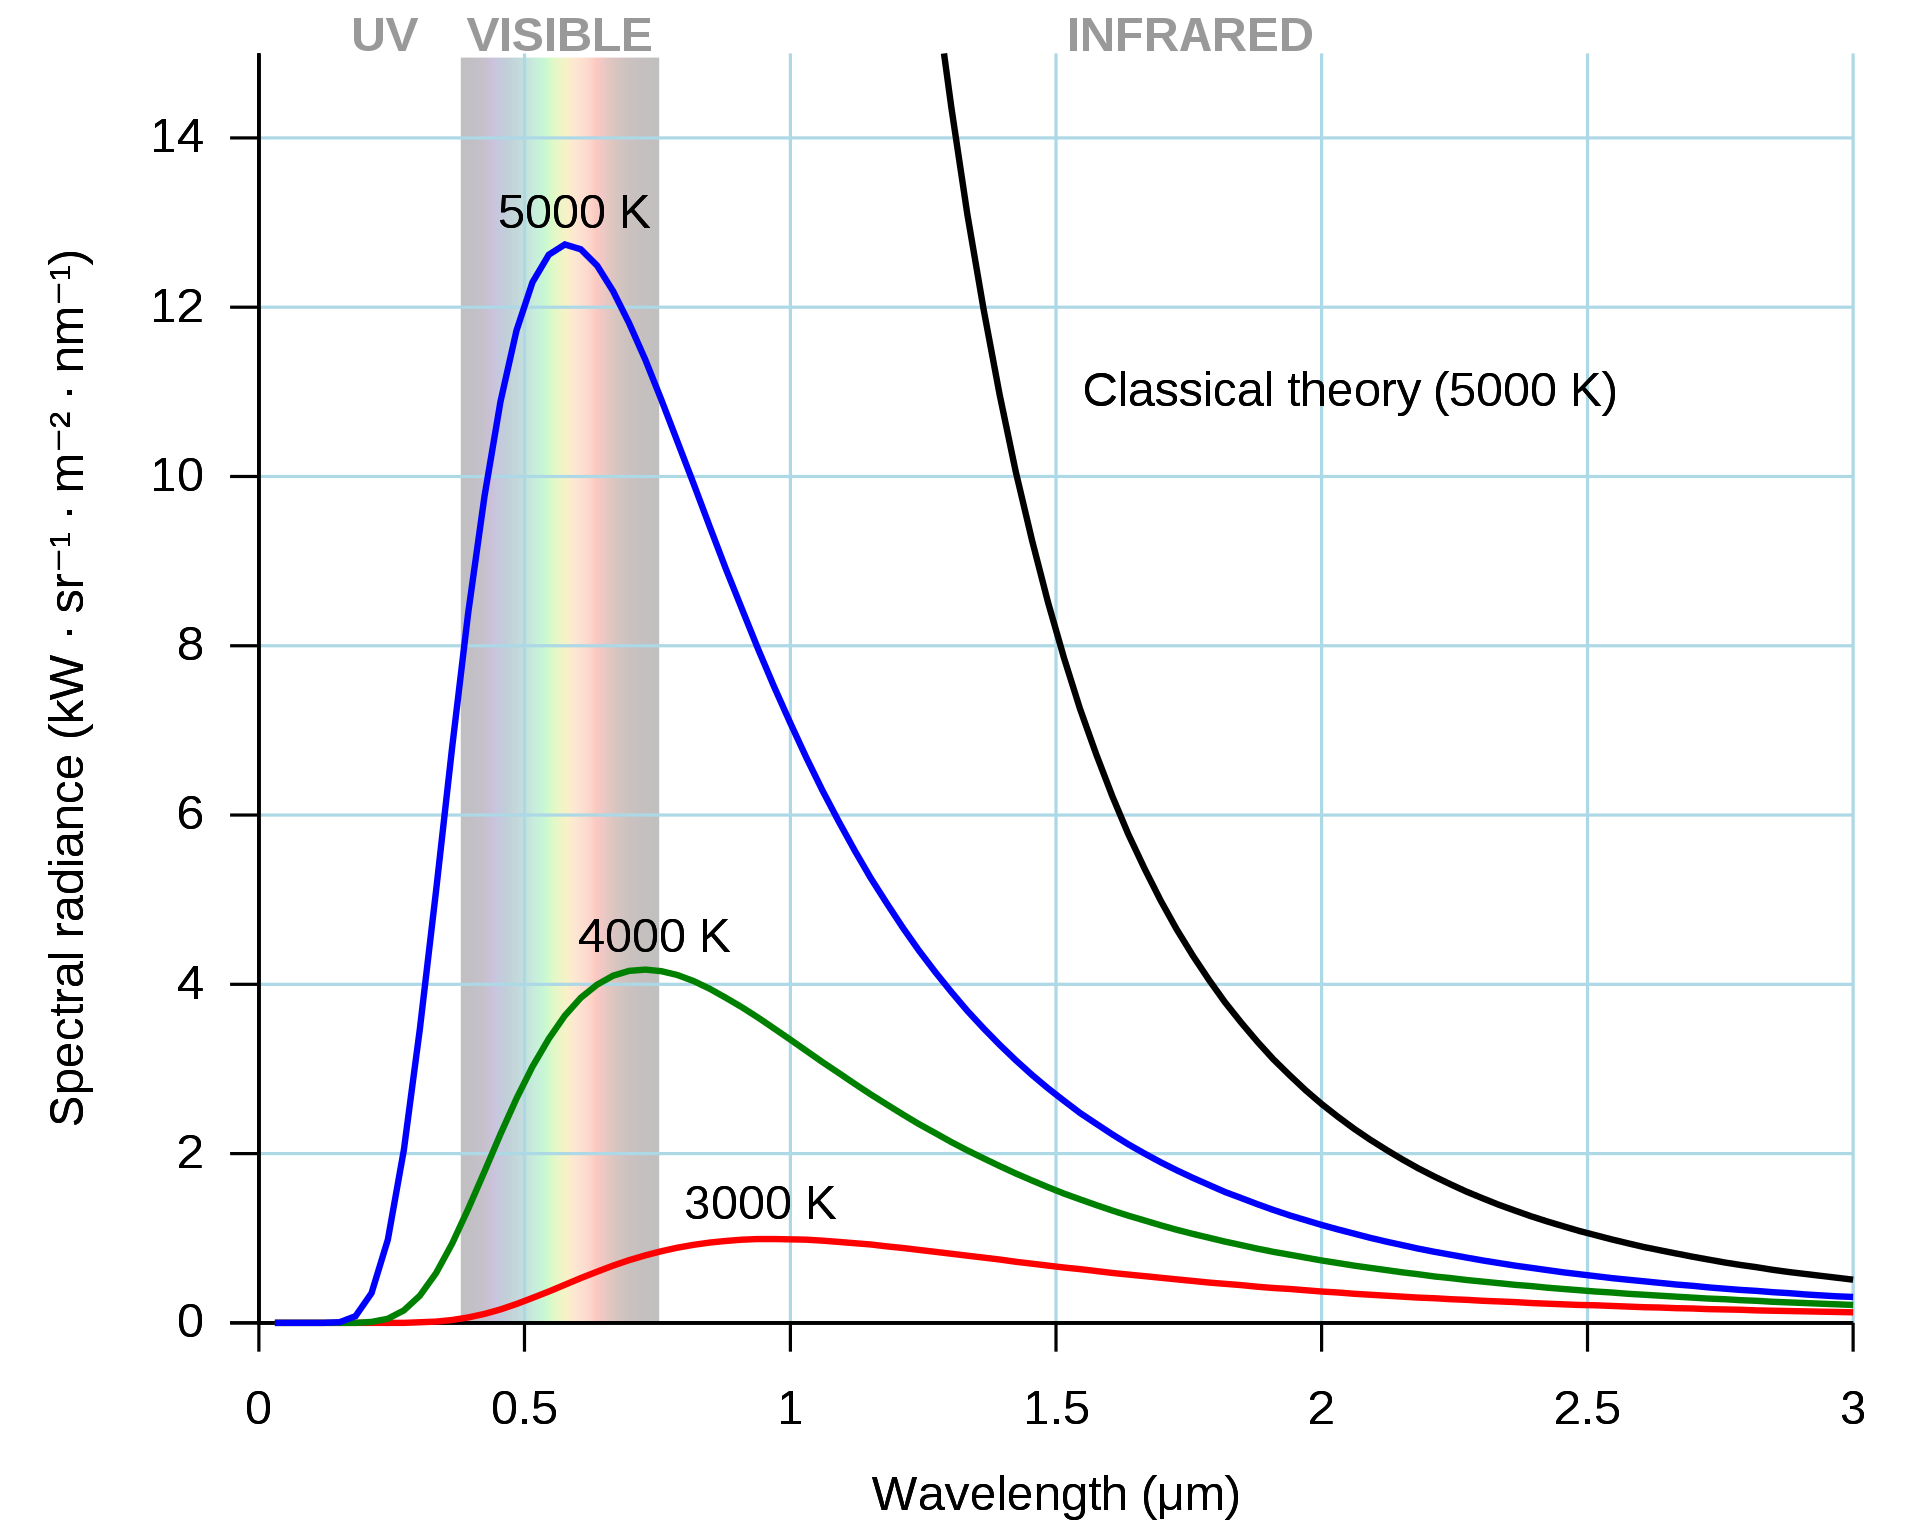
\includegraphics[width=\linewidth]{Wyk_1_Rys_5.png}
        \caption{Wykres promieniowania ciała doskonale czarnego}
        \label{lec_1:fig:cialo_doskonale_czarne}
    \end{figure}
    
    \begin{figure}[!ht]
        \centering
        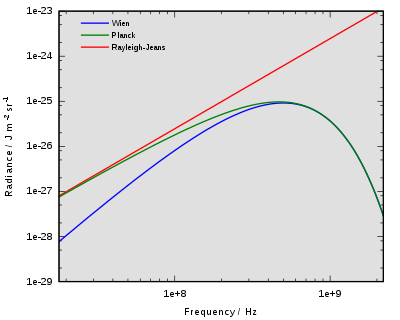
\includegraphics[width=\linewidth]{Wyk_1_Rys_6.png}
        \caption{Porównanie hipotezy Plancka z prawem Rayleigha-Jeansa i rozkładem Wiena. Further reading o 'Katastrofie w nadfiolecie'  na \link{https://pl.wikipedia.org/wiki/Ciało_doskonale_czarne}{Wikipedii o ciele doskonale czarnym}}
        \label{lec_1:fig:cialo_doskonale_czarne_porownanie}
    \end{figure}
    
    \subsection{Efekt Fotoelektryczny}
    \subsection{Analiza pól EM}
    Analiza pól $\E$ i B w odniesieniu do sześcianu z przewodnika prowadzi do wniosku, że energia "porcji promieniowania" transformuje się jak 
    \[\frac{\E'}{\E} = \frac{\sqrt{1 - \frac{u}{c}}}{\sqrt{1 + \frac{u}{c}}}\]
    gdzie $u$ - promieniowanie.
    Transformuje się to analogicznie do częstotliwości w efekcie Dopplera $\implies E \sim \nu$
    \\
    Rozkład energii będzie nam opisywać \ind{Rozkład Boltzmanna}, czyli rozkład prawdopodobieństwa zaobserwowania stanu Energetycznego, dany wzorem:
    \[p(E_i) \sim e^{-\frac{E_i}{k T}}\]
    co w przypadku rozkładu ciągłego daje nam zasadę ekwipartycji, ale dla dużych wartości energii się rozbiega z doświadczenie.
    
    \section{Skutki skwantowania energii}
    Przede wszystkim skutkiem jest \ind{indeterminizm}.\\
    
    \begin{figure}[!ht]
        \centering
        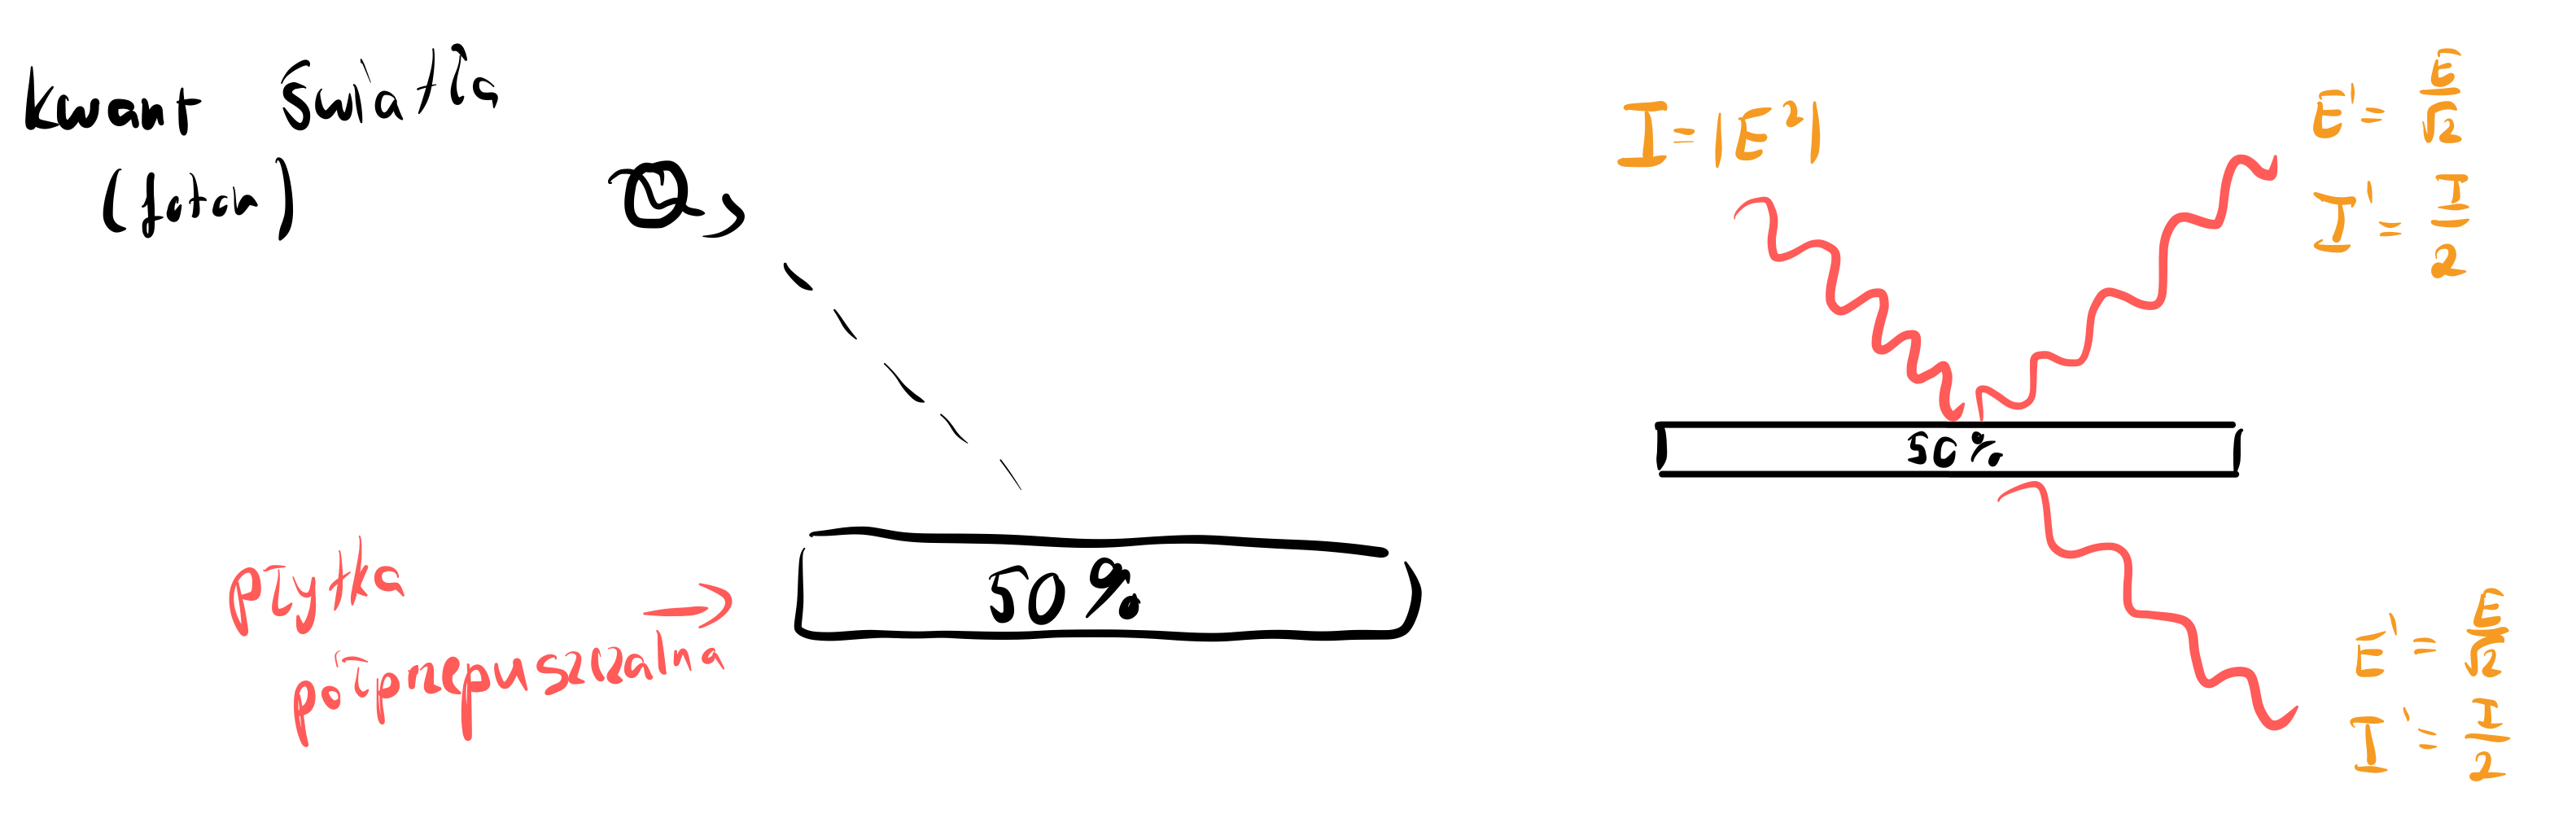
\includegraphics[width=\linewidth]{Wyk_1_Rys_1.jpeg}
        \caption{Demonstracja działania płytki półprzepusczalnej.}
        \label{lec_1:fig:plytka_polprzepuszczalna}
    \end{figure}
    
    \ind{Teoria parametrów ukrytych} - Teoria, że w kwantach energii występują nierejestrowane przez nas parametry, które jednakowoż zawsze determinują rozróżnienie kwantów energii. Parafrazując Drażana, dodawanie fotonom(kwantom) "włosów", "ogonów" itp - elementów rozróżniających je.\\
    
    Jeśli jednak nie chcemy dodawać fotonom 'włosów', ani 'ogonów' i chcielibysmy, żeby wszystkie fotony były "identyczne" to aby odtworzyć zachowanie klasyczne w granicy (podział natężenia 50\%), to musimy uznać, ze foton zachowuje się niedeterministycznie, tj. wprowadzić element probabilistyczny. Wtedy z prawdopodobieństwem 50\% każdy foton przechodzi lub odbija się.
    
    \begin{figure}[!ht]
        \centering
        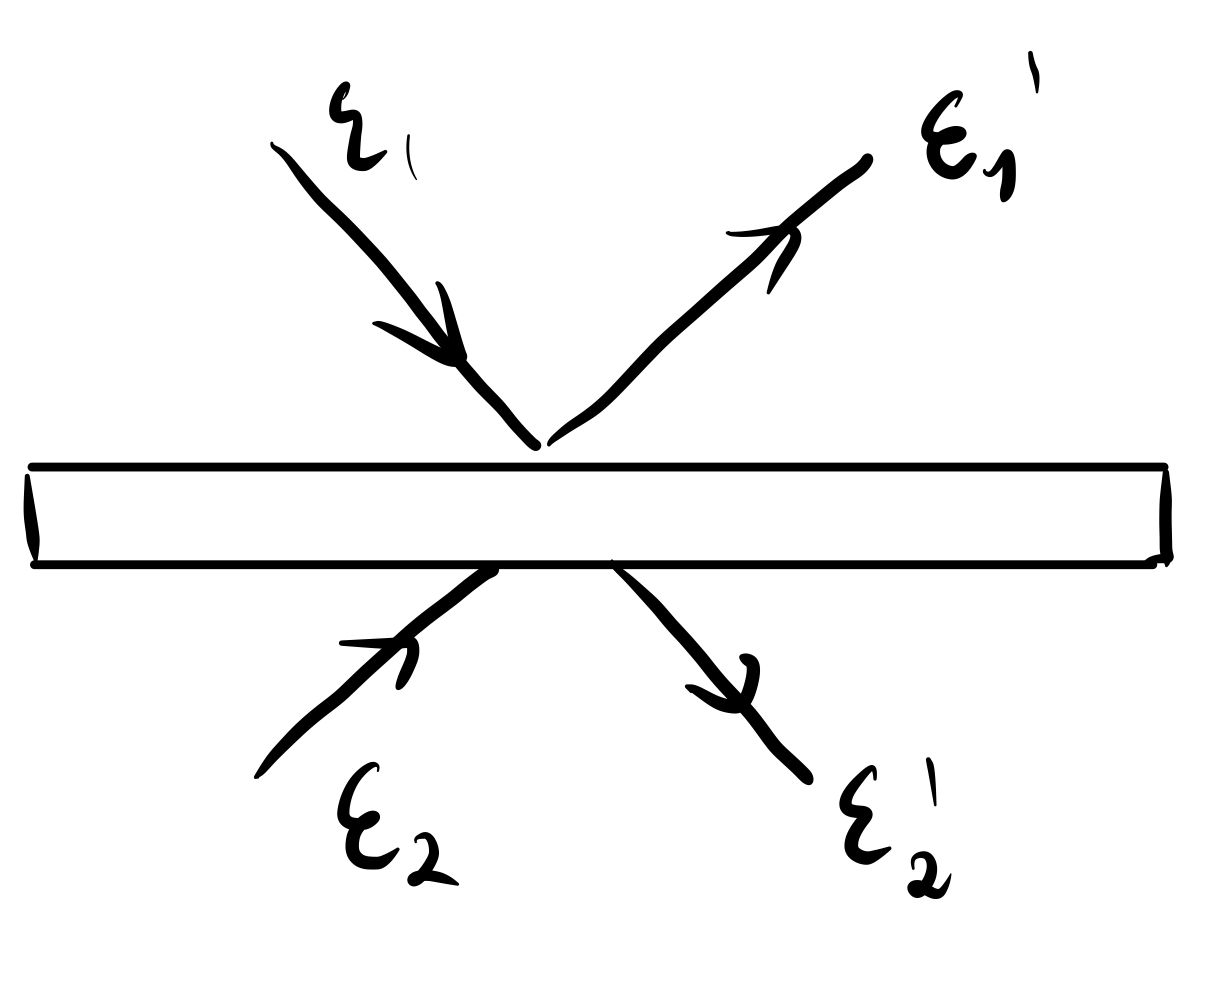
\includegraphics[width=0.6\linewidth]{Wyk_1_Rys_2.jpeg}
        \caption{Demonstracja działania płytki światłodzielącej ({\it Beam Splitter}).}
        \label{fig:lec_1:beam_splitter}
    \end{figure}
    
    Kiedy patrzymy na płytkę światłodzielącą (Rysunek \ref{fig:lec_1:beam_splitter}), to możemy przedstawiać bieg promienia w niej jako superpozycję fal (zapis macierzowy).
    \[\mqty[\E_1' \\ \E_2'] = B \mqty[\E_1 \\ \E_2] \implies \mqty[\R_1 & \T_2 \\ \T_1 & \R_2]\]
    Gdzie $\E_1' = \R1\E_1 + \T_2\E_2$. Chcemy, żeby \emph{energia była zachowana} \[\implies \vqty{\E_1}^2 + \vqty{\E_2}^2 = \vqty{\E_1'}^2 + \vqty{\E_2'}^2\]
    Co możemy też tłumaczyć jako zachowanie długości wektora $ \mqty[\E_1' \\ \E_2']$, czyli macierz $B$ jest macierzą \emph{Unitarną}, tj. $B\cdot B^\dag = 1$. 
    
    \[
        B B^\dag = \mqty[\R_1^\ast & \T_1^\ast \\ 
        \T_2^\ast & \R_2^\ast] 
        \cdot 
        \mqty[\R_1 & \T_2 \\ \T_1 & \R_2] = 
        \mqty[\vqty{\R_1}^2 + \vqty{\T_1}^2 & \R_1^\ast\T_2 + \T_1^\ast R_2 \\ 
        \R_1\T_2^\ast + \T_1 R_2^\ast & \vqty{\R_2}^2 + \vqty{\T_2}^2] = 
        \mqty[1 & 0 \\ 0 & 1]
    \]
    
    Wynika stąd, że $\vqty{\R_1}^2 = \vqty{\R_2}^2 = R$ - współczynnik odbicia natężenia, a $\vqty{\T_1}^2 = \vqty{\T_2}^2 = T$ - współczynnik transmisji natężenia, gdzie $R + T = 1$.
    
    W związku z tym też ogólnie mówiąc np.$ B = \mqty[\sqrt{R} & \sqrt{T} \\ -\sqrt{T} & \sqrt{R}]$, a $B_{50\%} = \frac{1}{2} \mqty[1 & 1 \\ -1 & 1]$. Tj. $B \in \mathcal{U}(2)$
    
    \section{Superpozycja}
    
    Pokażemy zjawisko interferencji w sensie kwantowym patrząc na kanoniczny przykład - \ind{Interferometr Macha-Zehndera}, widoczny na Rysunku \ref{fig:lec_1:interferometer}. Rozpatrujemy od teraz falę padającą postaci $\mqty[\E \\ 0]$.
    
    \begin{figure}[!ht]
        \centering
        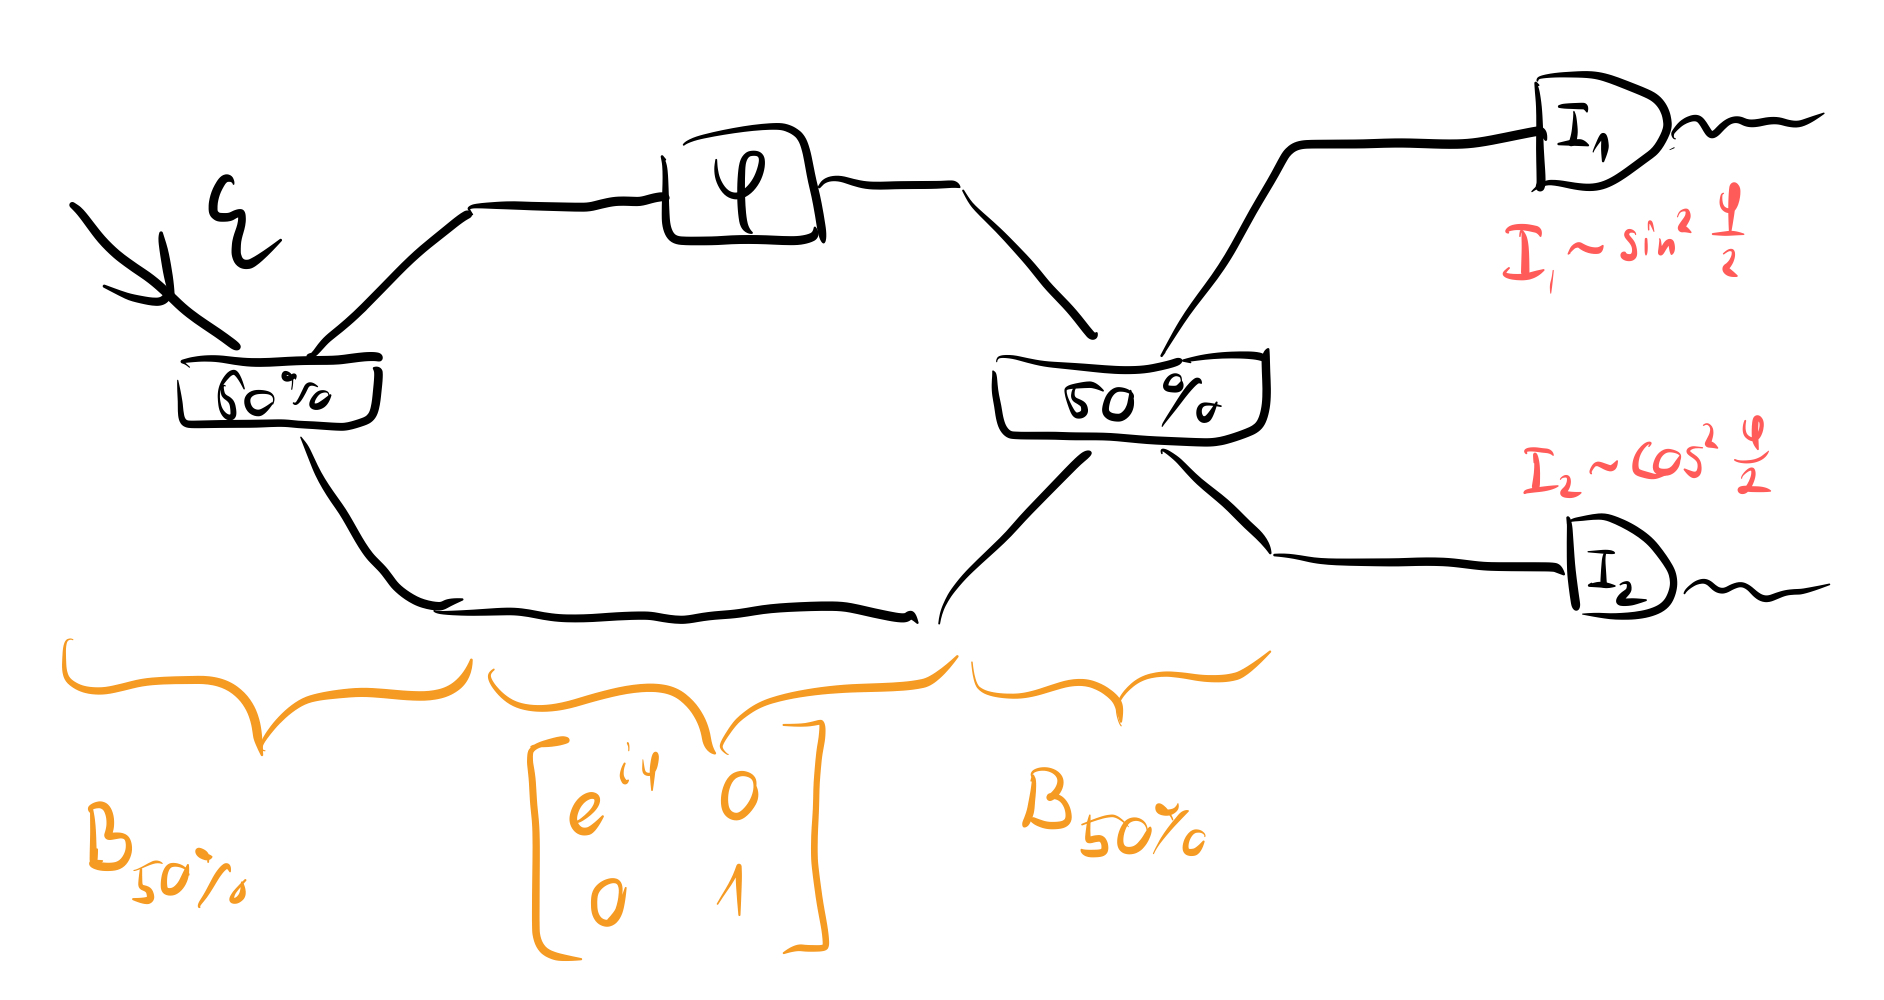
\includegraphics[width=0.8\linewidth]{Wyk_1_Rys_3.jpeg}
        \caption{Schemat konstrukcji Interferometru Macha-Zehndera wraz z podpisem macierzami Jonesa}
        \label{fig:lec_1:interferometer}
    \end{figure}
    
    \begin{figure}[!ht]
        \centering
        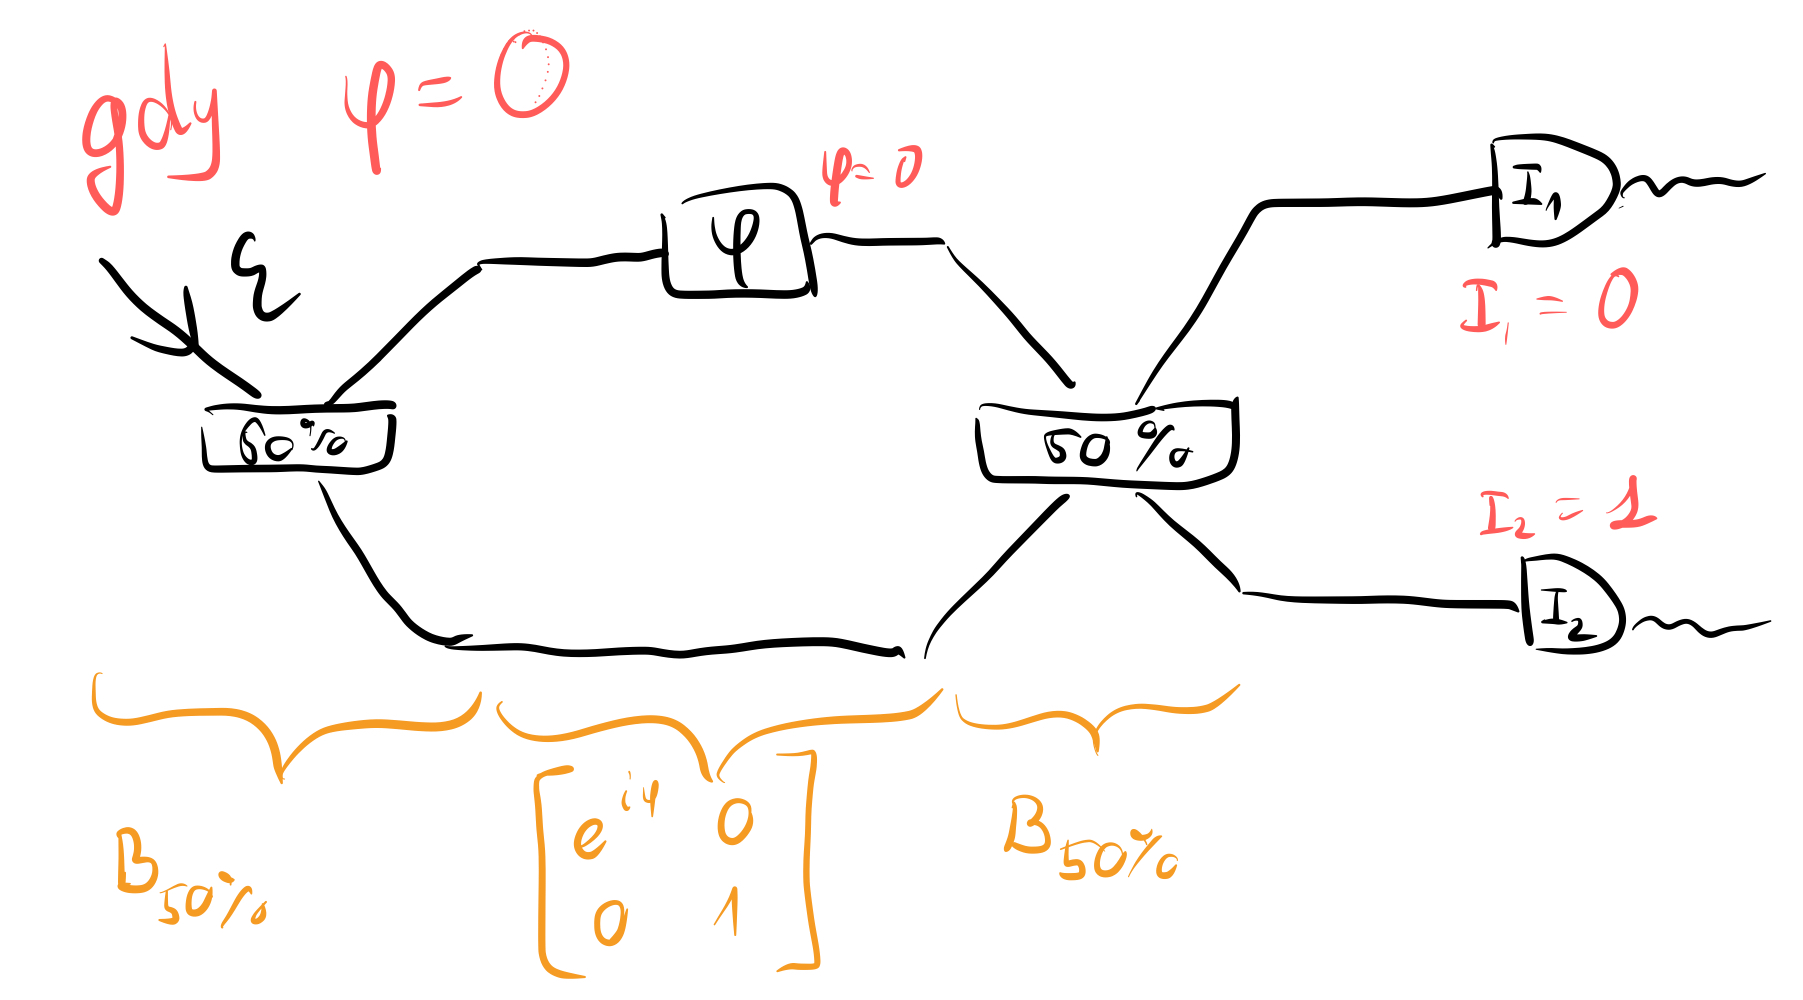
\includegraphics[width=0.8\linewidth]{Wyk_1_Rys_4.jpeg}
        \caption{Schemat konstrukcji Interferometru Macha-Zehndera wraz z podpisem macierzami Jonesa w przypadku zerowej zmiany fazy, tj. w szczególności dla jednego fotonu}
        \label{fig:lec_1:interferometer_phi_0}
    \end{figure}
    
    Teraz aby zrozumieć jak w takim układzie zachowuje się foton musimy odejść od klasycznego myślenia, że leci on jakąś drogą, a musimy przejść do myślenia o jego drodze jako \emph{nieokreślonej}, tj. do momentu wykonania pomiaru (wejścia w interakcję z nim) podąża on jednocześnie wszyskimi możliwymi dla siebie trajektoriami, tym samym przyjmując właściwości falowe. Da to efekt jak ten widoczny na Rysunku \ref{fig:lec_1:interferometer_phi_0}.
    
    Od teraz ten stan 'obierania wszystkich możliwości na raz' przez foton będziemy określać jako \subind{stan fotonu}{Stan!fotonu} oznaczany $\ket{\Psi}$. Tłumaczy się to na funkcję gęstości prawdopodobieństwa znalezienia fotonu w jego możliwych trajektoriach.
    
    W szczególności w opisywanym wyżej przypadku stan $\ket{\Psi}$ będzie opisywany przez \emph{superpozycję} stanów 1 i 2 odpowiadających pójściem drogą odpowiednio górną i dolną, tj. $\ket{\Psi} = \mqty[\Psi_1 \\ \Psi_2]$ gdzie $\Psi_i$ - aplituda prawdopodobieństwa obrania ścieżki $i$, a $p_i = \qty|\Psi_i|^2$ - prawdopodobieństwo, że foton leci i-tą trajektorią.
    
    \begin{equation}
        \ket{\Psi} = \Psi_1\ket{1} \oplus \Psi_2 \ket{2}
        \label{eq:lec_1:superpozycja}
    \end{equation}
    
    Gdzie znakiem $\oplus$ oznaczamy dodawanie fal. Ta operacja to \ind{Superpozycja}. Warto też zanotować, że skoro $\qty|\Psi_i| = p_i$ to ich suma musi się dodawać do 1 
    \[
        \sum_i \qty|\Psi_i|^2 = 1
    \]
    ({\it innymi słowy prawdopodonbieństwo znalezienia fotonu w całej przestrzeni zdarzeń jest 1})
    
    Dla zbudowania intuicji na ten moment możemy sobie utożsamiać tę funkcję pradopodobieństwa z obserwowanym natężeniem światła:
    \[
        \qty|\Psi_i|^2 \sim \qty|\E_i|^2 \sim I_i
    \]
    
\section{Hipoteza De Broigle'a}
{\it Side note 1}: W naszych rozważaniach nie będzie mieć znaczenia faza całkowita, znaczenie będzie mieć tylko faza względna między ramionami, tj. $\E_i \to e^{i \xi} \E_i$. Innymi słowy, 'globalna faza' {\color{brown} nie istnieje!.}

Wyszliśmy w naszych dywagacjach od myślenia o fotonach jako o obiektach falowych, ale nie można zapomnieć o tym, że fotony mają również właściwości korpuskularne, więc sugeruje to, że dla materii też to powinno działać. W związku z tym \ind{Hipoteza De Broigle'a} odpowiadać nam będzie za opisanie 'fal materii', gdzie ich długość fali to będzie:
\[
    \lambda = \frac{h}{p}
\]
Co dla światła ma interpretację:
\[
    p = \frac{E}{c} = \frac{h \cdot \mu}{c} = \frac{h}{\lambda}
\]
Gdzie $E$ - Energia.
    
    Further reading: 
    \begin{itemize}
        \item \link{http://studenci.fuw.edu.pl/~kc427902/Prezentacje_Kwanty/wyklad1-foton.pdf}{Notatki Demko do tego wykładu}
        \item \link{http://studenci.fuw.edu.pl/~kc427902/Prezentacje_Kwanty/cwiczenia1.pdf}{Zadanka na ćwiczenia 1}
        \item \link{http://studenci.fuw.edu.pl/~kc427902/Prezentacje_Kwanty/cwiczenia1.pdf}{Zadanka na ćwiczenia 2}
    \end{itemize}
\end{lecture}

% ------------------------------------------------------------------------
% Wykład 04.03.2022

\begin{lecture}{Stany i pomiary kwantowe}

\section{Stany i pomiary kwantowe}
W tym wykładzie zajmiemy się powoli formalizowaniem intuicji nabywanej na poprzednim wykładzie. Zdefiniujmy $\ket{i}$ - pewne stany rozróżnialne (istnieje pomiar dający róne wyniki dla różnych stanów).

\begin{emph_box}{\subind{Zasada superpozycji}{Zasada!superpozycji}}
Jeśli $\ket{1}$ i $\ket{2}$ są dopusczalnymi stanami układu, to "$\ket{1}\oplus\ket{2}$"\footnote{rozumiemy to jako "jednocześnie $\ket{1}$ i $\ket{2}$"} też musi być dopuszczalnym stanem układu
\end{emph_box}

Matematyczna struktura odpowiednia dla superpozycji to:
\begin{itemize}
    \item Przestrzeń Hilberta $\HS$ nad $\CS$
    \item $\HS$ - przestrzeń wektorowa nad $\CS$ z iloczynem skalarnym $\braket{\Psi}{\phi}$, $\ket{\Psi} \in \HS$\footnote{wektor reprezentuje stan}, zupełna\footnote{każdy ciąg Cauchy zbiega do elementu $\HS$}
    \item \uwaga{każda skończenie wymiarowa przestrzeń Hilberta (dim $\HS = d$) jest izomorficzna z $\CS^d$}.
\end{itemize}

\subind{Stan Kwantowy}{Stan!kwantowy}:
Niech $\ket{\Psi} \in \HS$, $\braket{\Psi} = 1$. \uwaga{$\ket{\Psi} \phys e^{i \xi} \ket{\Psi} \implies \ket{\Psi} \phys z \cdot \ket{\Psi}$\footnote{Symbol $\phys$ oznacza 'w interpretacji fizycznej ...'}}\\
Stanem kwantowym nazwiemy też promień w przestrzeni Hilberta $\HS$

\ind{Pomiary kwantowe}:
W przestrzeni Hilberta $\HS$ bierzemy sobie wektory $\ket{a_i} \in \HS$, tworzące bazę ortonormalną w $\HS$. Bedzie to zespół rozróżnialnych stanów różniących się pewną obserwowalną wielkością ficzyną $A$. Czyli przyjmujemy:\\
$\ket{a_i}$ - mają dobrze określoną wartośc wielkości fizycznej $A$. Zawsze jak je mierzymy to dostajemy $a_i$.\\
Innymi słowy, jak mamy kilka wielkości fizycznych $A, B, C, \dots$, to w ogólności {\color{red} nie będziemy mogli znaleźć jednej bazy ortonormalnej} $\ket{a_i, b_i, c_i, \dots}$. Jest to esencja mechaniki kwantowej, że różne wialkości fizyczne związane są z różnymi, niekompatybilnymi wobec siebie bazami, które opisują każdą z osobna.\footnote{Czyli pomiar$\neq$zaglądanie do garnka /sprawdzanie stanu który jest zdeterminowany/}

    \begin{figure}[!ht]
        \centering
        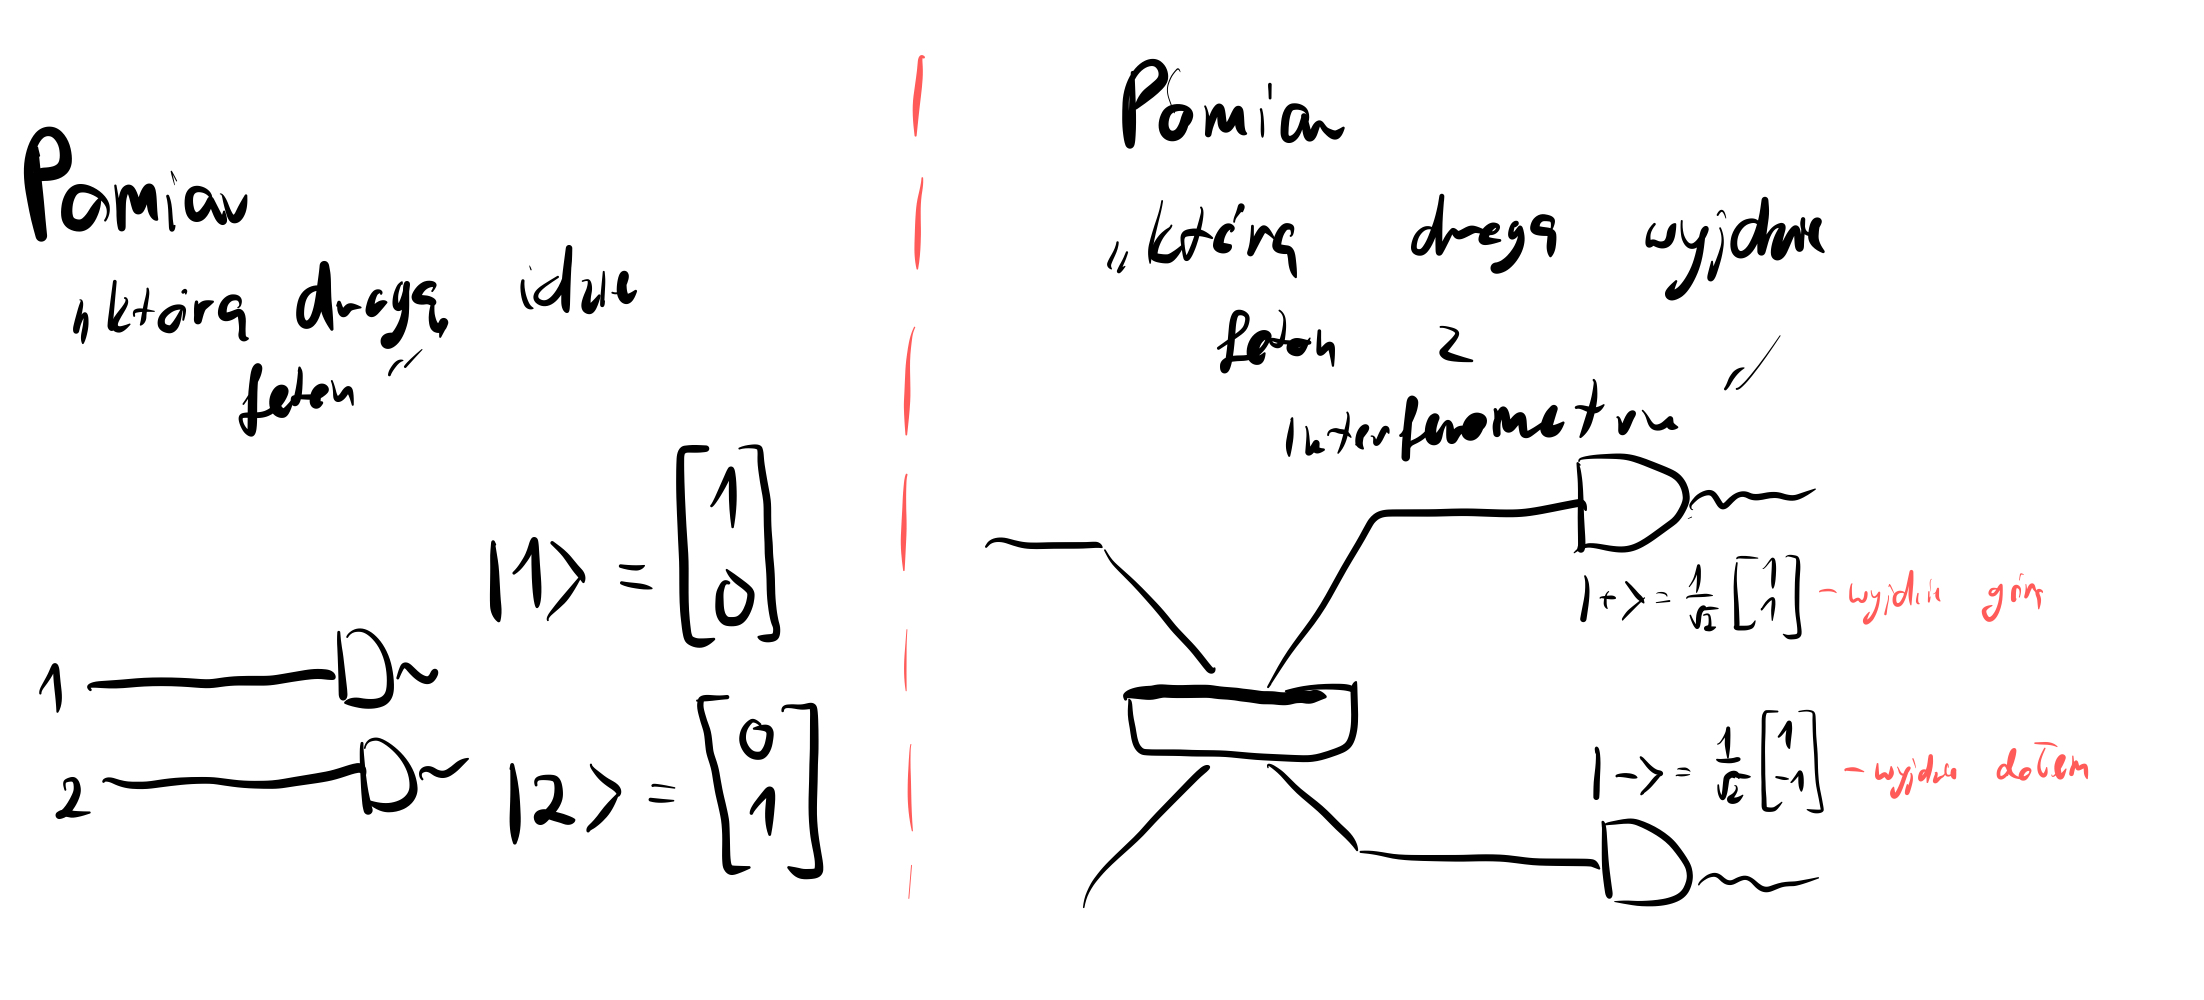
\includegraphics[width=0.8\linewidth]{Wyk_2_Rys_1.jpeg}
        \caption{Porównanie podejść myślenia o kwantu - deterministyczny i niedeterministyczny}
        \label{fig:lec_2:porownianie}
    \end{figure}
    

\begin{emph_box}{\ind{Postulat pomiarowy}}
    Jeśli $\ket{\Psi}$ jest dowolnym stanem, na którym chcemy zmierzyć wielkość fizyczną $A$, z którą stowarzyszona jest baza $\qty{\ket{a_i}}$. Możemy napisać:
    \[\ket{\Psi} = \sum_i \alpha_i\ket{a_i}\]
    Wtedy uzyskany wynik $a_i$ z prawdopodobieństwem $p_i = \qty|\alpha_i|^2 = \qty|\braket{a_i}{\Psi}|^2$. Tym samym stan po pomiarze ma dobrze określone wielkości $a_i$, tj. jest $\ket{\Psi} = \ket{a_i}$.
\end{emph_box}
 Czyli też jak już raz dokonamy pomiaru na stanie kwantowym to on już nie wróci do możliwości interferencji, i za każdym kolejnym pomiarem już będziemy obserwować ten sam stan, tj. zacznie się zachowywać jakby był klasyczny.
    
\ind{Observabl-a}:
Z pomiarem wielkości A $\qty(\qty{\ket{a_i}})$ stowarzyszamy operator 
\[
    \hat{A} = \sum_i a_i \ketbra{a_i}
\]
gdzie $\hat{A}$ jest operatorem Hermitowskim\footnote{Operator hermitowski - $A^\dagger = A$} czyli w szczególności mając $\hat{A}$ możemy też znaleźć $\qty{\ket{a_i}}$ robiąc rozkład własny.

\begin{align*}
\hline \hline
\end{align*}

{\it Crash course z notacji Diraca:}\\
\textbf{ket}:
\[
    \ket{a} = \mqty[a_1 \\ a_2 \\ \vdots \\ a_n] = \vb{v}
\]
\textbf{bra}:
\[
    \bra{a} = \ket{a}^\dagger = \mqty[a_1, a_2, \cdots, a_n]^\ast = \vb{v}^\dagger
\]
Czyli jak je połączymy dostajemy \textbf{braket}:
\[
    \braket{a}{b} = \mqty[a_1, a_2, \cdots, a_n]^\ast \cdot \mqty[b_1 \\ b_2 \\ \vdots \\ b_n] = \vb{v} \cdot \vb{v}^\ast = liczba\footnote{Iloczyn skalarny}
\]
Zaś z kolei jak pomnożymy w odwrotnej koleności mamy \textbf{ketbra}:
\[
    \ketbra{a}{b} =  \mqty[a_1 \\ a_2 \\ \vdots \\ a_n] \cdot \mqty[a_1, a_2, \cdots, a_n]^\ast = M \in M(\CS)_n^n
\] co rozumiemy też jako operator rzutowy.

\begin{align*}
\hline \hline
\end{align*}

Obserwable jest wygodniej liczyć jako wartości oczekiwane z jakichś rozkłądów prawdopodobieństw:\\
\[
    \expval{A} = \sum_i p_i a_i = \sum_i \qty|\braket{a_i}{\Psi}|^2 \cdot a_i
\]
Gdzie wiemy, że człon $\qty|\braket{a_i}{\Psi}|^2$ możemy rozpisać jako:
\[
    \qty|\braket{a_i}{\Psi}|^2 = \qty|\braket{\Psi}{a_i}|^2 = \braket{\Psi}{a_i}\braket{a_i}{\Psi} = \bra{\Psi} \quad \ketbra{a_i} \quad \ket{\Psi}
\]
W związku z tym możemy dalej rozpisać $\expval{A}$ jako:
\[
    \expval{A} = \bra{\Psi} \quad \sum_i a_i \ketbra{a_i} \quad \ket{\Psi} =\footnote{${\color{blue} \sum_i a_i \ketbra{a_i} = \hat{A}}$} \ev{\hat{A}}{\Psi}
\]

Further reading:
\begin{itemize}
    \item \link{http://studenci.fuw.edu.pl/~kc427902/Prezentacje_Kwanty/wyklad2-stanypomiary.pdf}{Notatki Demko do wykładu}
    \item \link{http://studenci.fuw.edu.pl/~kc427902/Prezentacje_Kwanty/cwiczenia2.pdf}{Zadania na ćwiczenia 2}
    \item \link{http://studenci.fuw.edu.pl/~kc427902/Prezentacje_Kwanty/cwiczenia2-sol.pdf}{Rozwiązania z ćwiczeń 2}
\end{itemize}
\end{lecture}

% --------------------------------------------------------
% Wykład 09.03.2022

\begin{lecture}{Ewolucja stanów kwantowych i Hamiltonian}
\section{Ewolucja stanów kwantowych}
Będziemy brać teraz pod uwagę tylko \emph{układy izolowane}! Tutaj rozumiemy, że \ind{Układ izolowany} - układ który nie oddziaływuje z otoczeniem i brak pomiarów.\\
Formalnie napiszemy, że (póki co bez żadnych założeń) $\ket{\Psi(0)}$ - stan w chwili początkowej, $\ket{\Psi(t)}$ - stan po czasie. Teraz chcemy wiedzieć, jaki będzie $\ket{\Psi(t)}$?
Otóż:
\[
    \ket{\Psi(0)} = \mathcal(U)(t)\qty[\ket{\Psi(0)}]
\]
Tj. tak jak w mechanice klasycznej - założymy, że nasza ewolucja w czasie jest odwracalna. Wynika z tego, że 
\begin{itemize}
    \item \emph{stany rozróżnialne\footnote{Ortogonalne} muszą pozostać rozróżnialne.} Możemy na to patrzeć jako na \emph{zachowanie informacji}.
    \[
        \braket{\Psi(0)} = 0 \qc \braket{\Psi(t)} = 0
    \]
    \item Stopień rozróżnialności tych stanów zależeć będzie od ich iloczynu skalarnego. Chcemy, żeby pozostał on stały $$\implies \braket{\Psi(0)} = \braket{\Psi(t)}$$
\end{itemize}

{\color{teal} Fakt}: $U(t)$ jest liniowe.\\
Sprawdźmy go. Także rozważmy $$\ket{\xi} = U(t)\qty[a \ket{\Psi(0)} + b \ket{\Psi(0)}] - a U(t)\qty[\ket{\Psi(0)}] - b U(t)\qty[\ket{\Psi(0)}]$$
Teraz obliczmy:
\begin{align*}
    \braket{\xi} &= \qty(U(t) \qty[a \psket{0} + b \psket{0}])^\dagger \qty( U(t) \qty[a \ket{\Psi(0)} + b \ket{\Psi(0)}] - a U(t) \qty[\ket{\Psi(0)}] - b U(t) \qty[\ket{\Psi(0)}])\\
    &- \qty(a U(t) \qty[\psket{0}])^\dagger \qty(-||-)\\
    &- \qty(a U(t) \qty[\psket{0}])^\dagger \qty(-||-)
\end{align*}
Czyli $\qty(U(t)\ket{\Psi})^\dagger (U(t) \ket{\Psi}) = \braket{\Psi} = 0$, bo można 'usunąć' wszystkie $U(t)$. Wynika z tego, że $U(t)$ \emph{jest liniowe.}

{\color{teal} Wnioski}: $U(t)$ jest liniowa (w skończenie wymiarowych przestrzeniach reprezentowanych przez macierz\footnote{Bo $(AB)^\dagger = A^\dagger B^\dagger$}) i zachowuje iloczyn skalarny.
\[
    \implies \psket{0} = U(t) \cdot \psket{0}
\]

Teraz ciągnąc to rozumowanie dalej:
\[
    \forall_{\ket{\Psi(0)}, \ket{\varphi(0)}} = \braket{\Psi(0)}{\varphi(0)} = \mel{\Psi(0)}{U^\dagger(t) U(t)}{\varphi(0)} = \braket{\Psi(0)}{\varphi(0)}
\]
Wynikać z tego będzie, że $U(t)^\dagger U(t) = 1$. Wiedząc, że pracujemy w skończenie wymiarowej przestrzeni wnioskujemy, że $U(t)$ jest \emph{Unitarne}. Oznacza to też, że $U^{-1}(t) = U(t)^\dagger$. Teraz fizycznym argumentem, że $U^{-1}(t)$ istnieje będzie to, że powinno być $U^{-1}(t) = U(-t)$.\\

Idziemy dalej. Wiemy, że $U(t=0) = \Id$. Rozważmy pierwsze (liniowe) rozwinięcie $U(t)$ w czasie:
\[
    U(dt) = \Id + \qty(- \frac{i}{\hbar} H \dd{t} + O(\dd{t}^2))
\]
\[
1 = U(\dd{t})^\dagger U(\dd{t}) = \qty(\Id + \frac{i}{\hbar} H^\dagger \dd{t} + O(\dd{t}^2)) \qty(\Id - \frac{i}{\hbar} H^\dagger \dd{t} + O(\dd{t}^2)) = \Id + \frac{i}{\hbar} (H^\dagger - H) \dd{t} + O(\dd{t}^2)
\]
Czyli widzimy, że $H^\dagger = H$ - jest Hermitowskie.

\[
    \psket{\dd{t}} = U(\dd{t}) \psket{0} = \psket{0} - \frac{i}{\hbar} H \dd{t} \psket{0} + O(\dd{t^2}) = \psket{0} + \dv{\psket{t}}{t}\eval_{t=0} + \order{\dd{t^2}}
\]
\[
    \dv{\psket{t}}{t}\eval_{t=0} = - \frac{i}{\hbar} H \psket{0} \implies i \hbar \dv{\psket{t}}{t}\eval_{t=0} = H \psket{0}
\]Ale zamiast pisać $\psket{\dd{t}} = U(\dd{t}) \psket{0}$ można ogólniej powiedzieć: $\psket{t + \dd{t}} = U(\dd{t}) \psket{t}$.\\
Dostajemy krypto \ind{Równanie Schrödingera}:
\begin{equation}
    i \hbar \dv{\psket{t}}{t} = H \psket{t}
    \label{eq:lec_3:krypto_schrodinger}
\end{equation}
(Krypto, bo nie znamy natury $H$)

\section{Argument za naturą fizyczną H}
Rozważmy obserwablę $A$ i jej wartość oczekiwaną na stanie $\psket{t}$.
Wtedy:
\[
    \ev{A}_t = \ev{A}{\Psi(t)}
\]
\begin{align*}
    \dv{\ev{A}_t}{t} &= \dv{\bra{\Psi(t)}}{t} A \psket{t} + \ev{A}{\Psi(t)} = \frac{i}{\hbar} \ev{H\cdot A - A \cdot H}{\Psi(t)}\\
    &= \frac{i}{\hbar} \ev{\qty[H, A]}{\Psi(t)} = - \frac{i}{\hbar} \ev{\qty[A, H]}{\Psi(t)}
\end{align*}

Jeśli wybierzemy $A = H \implies \dv{\ev{H}}{t} = 0$ czyli H jest związany z wielkością fizyczną zachowaną w czasie ewolucji $\implies$ w
pierwsza myśl, że ma coś wspólnego z energią.

\begin{emph_box}{Analogia z Mechaniką Klasyczną}
$$A(q, p) \qc \dv{A}{t} = \qty{A, H} = \sum_i \dv{A}{q_i} \dv{H}{p_i} - \dv{A}{p_i}\dv{H}{q_i}$$
Formalna recepta wiążąca mechanikę klasyczną z kwantową: $$\qty{\cdot, \cdot} \to =-\frac{i}{\hbar} \qty[\cdot , \cdot]$$
Jest to dodatkowy argument na to, że H ma coś wspólnego z energią.
\end{emph_box}

To teraz dochodzimy do równań:
\[
    \dv{\psket{t}}{t} = - \frac{i}{\hbar} H \psket{t} \implies \psket{t} = U(t) \psket(0)
\]
Gdzie $U(t) = e^{- \frac{i}{\hbar}H \cdot  t}$
Gdzie wreszcie piszemy, że H - Hamiltonian.

\section{Wyznaczenie ewolucji stanu w praktyce}

Mamy $H$, robimy jego rozkład własny, tj. $H = \sum_k E_k\footnote{Wartości własne (energie)}\ketbra{E_k}$. $H\ket{E_k} = E_k\ket{E_k}$

Jeśli:\\
$\psket{0} = \ket{E_k}, \qq{stan o dobrze określonej energii}$\\
$\psket{t} = e^{- \frac{i}{\hbar}H \cdot  t} \ket{E_k} = e^{- \frac{i}{\hbar}E_k \cdot  t} \ket{E_k}$\\
Czyli energia stanu o dobrze określonej energii zmienia tylko globalną fazę, czyli fizycznie stan się nie zmienia.\\
Ogólnie jeśli mamy dowolny stan początkowy $\psket{0}$, to możemy go rozłożyć w bazie $\qty{\ket{E_k}}$. W takim razie widzimy, że zajdzie:\\
$\psket{0} = \sum_k c_k\footnote{$c_k = \braket{E_k}{\Psi(0)}$} \ket{E_k}$, z liniowości $\psket{t} = \sum_k c_k U(t)\ket{E_k} = \sum_k c_k e^{- \frac{i}{\hbar}E_k \cdot t} \ket{E_k}$\\
\emph{Uogólnienie} W modelach gdy $H$ zależy jawnie od czasu (czyli de facto bierzemy układ izolowany) możemy te układy wciąż opisywać jakby były izolowane, ale musimy dopuścić $H = H(t)$. Wtedy jedyna zmiana jaka się pojawia, to:
\[
    \dv{\psket{t}}{t} = - \frac{i}{\hbar} H(t) \psket(t) \implies U(t) \approx e^{- \frac{i}{\hbar} (t - \Delta t) \Delta t} \dots e^{- \frac{i}{\hbar} (\Delta t) \Delta t} e^{- \frac{i}{\hbar} (0) \Delta t}
\]
\[
    U(t) \approx
    \begin{cases}
        U(t) = e^{- \frac{i}{\hbar} \int_0^t H(t) \dd{t}}, \qq{jeśli H(t) komutują ze sobą w różnych chwilach czasu}\\
        U(t) = \tau\footnote{uporządkowanie czasowe} \qty[e^{- \frac{i}{\hbar} \int_0^t H(t) \dd{t}},]
    \end{cases}
\]
\end{lecture}

% --------------------------------------
% 11.03.22

\renewcommand{\psket}[1]{\ket{\Psi(#1)}}

\begin{lecture}{Równanie Schrodingera (na koszulkach)}
\section{Schizofreniczna Ewolucja}

\begin{figure}[!ht]
        \centering
        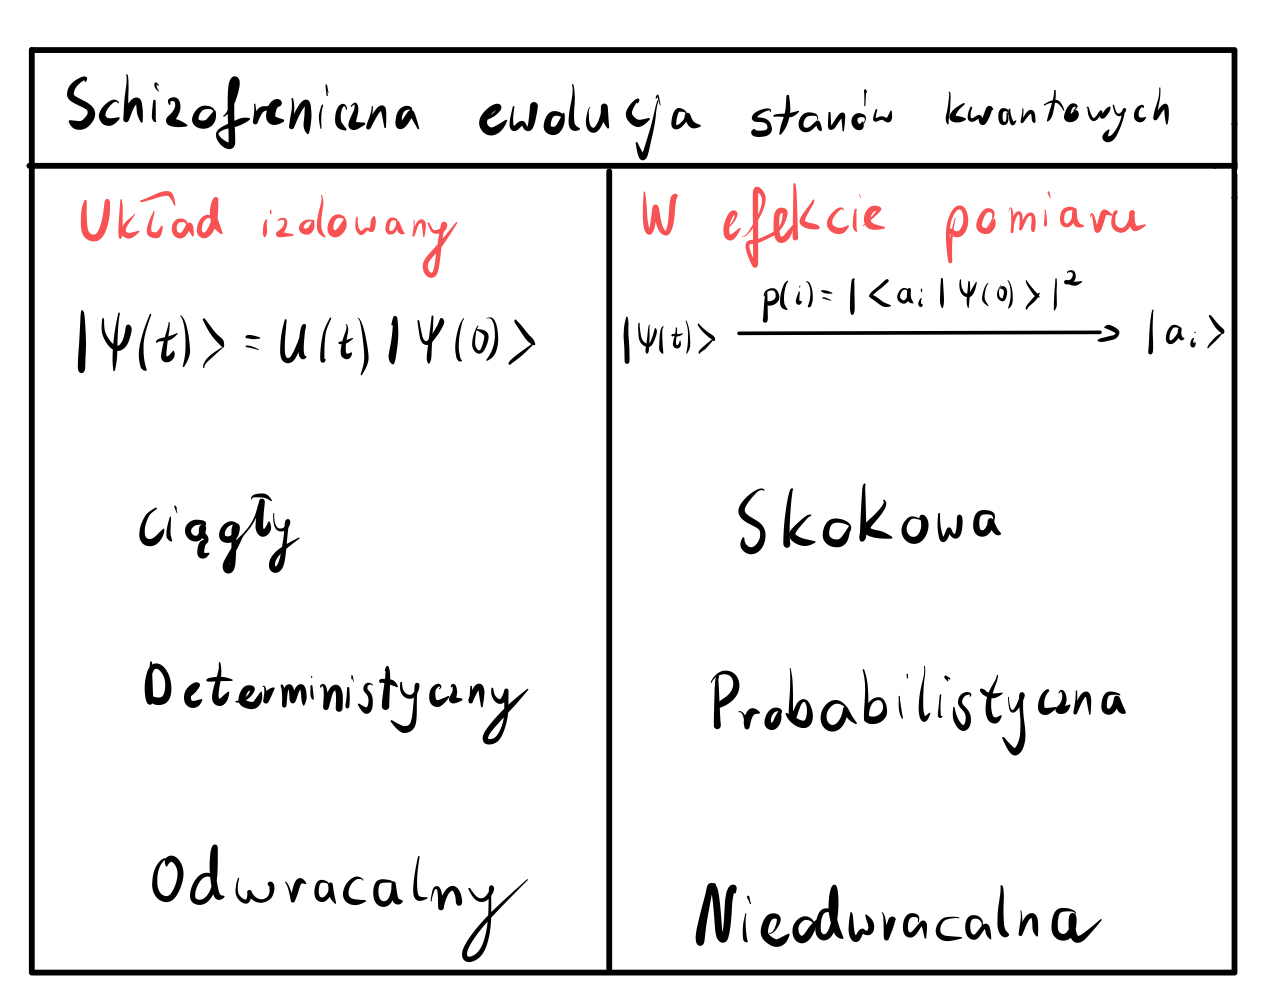
\includegraphics[width=\linewidth]{Wyk_4_Rys_1.jpeg}
        \caption{Schizofreniczna Ewolucja}
        \label{lec_4:fig:tabelka}
\end{figure}

\section{Kwantowy Efekt Zenona (z Elei)}
Formułował wiele paradoksów - miał dobrą intuicję. Jeden z bardziej znanych - \emph{paradoks strzały}\\
\textit{Paradoks strzały} - Skoro strzała w każdej chwili spoczywa, to ruch jest niemożliwy.

Rozważmy układ kwantowy, którego ewolucja jest opisana Hamiltonianem $\HS$.
\begin{itemize}
    \item Stan początkowy $\psket{0}$ nie będzie stanem własnym $\HS$ (żeby ewoluował nietrywialnie).
    \item Wtedy ewolucja po czasie $t$: $\psket{t} = e^{- \frac{i\HS t}{\hbar}}\psket{0}$ i sprawdzamy, czy układ wciąż jest w stanie $\psket{0}$ \footnote{Czyli wykonujemy pomiar w bazie ortonormalnej, której jednym z wektorów jest $\psket{0}$}
    \item Prawdopodobieństwo, że stan pozostał niezmieniony: \\$p(t) = \qty|\braket{\Psi(0)}{\Psi(t)}|^2 = \braket{\Psi(0)}{\Psi(t)}\braket{\Psi(t)}{\Psi(0)} = \ev{e^{- \frac{i\HS t}{\hbar}}}{\Psi(0)} = \ev{e^{\frac{i\HS t}{\hbar}}}{\Psi(0)}$\\
    Wtedy po rozwinięciu dla małych $t$ \footnote{$e^x \approx 1 + x + \frac{x^2}{2} + \order{x^3}$}:
    \begin{align*}
        p(t) &= 1 + t \cdot \qty[\ev{- \frac{i\HS}{\hbar}}{\Psi(0)} \braket{\Psi(0)} + \braket{\Psi(0)} \ev{\frac{i\HS}{\hbar}}{\Psi(0)} ] + \\
        &- t^2\cdot \qty[\ev{\frac{\HS^2}{\hbar^2}}{\Psi(0)} \braket{\Psi(0)} + \frac{1}{2} \braket{\Psi(0)} \ev{\frac{\HS^2}{\hbar^2}}{\Psi(0)} - \ev{\frac{\HS}{\hbar}}{\Psi(0)}\ev{\frac{\HS}{\hbar}}{\Psi(0)}] + \order{t^3} \\
        &= 1 + \frac{t^2}{\hbar^2} \underbrace{(\ev{\HS^2}{\Psi(0)} - \ev{\HS}{\Psi(0)}^2)}_{\Delta^2 \HS\footnotemark} + \order{t^3}
    \end{align*}
    \footnotetext{Stan ewoluuje 'tym szybciej' im ma większą ma wariancję $\HS$}
    Czyli wyobrażamy sobie, że mierzymy stan coraz częściej, czyli n razy co czas $\frac{t}{n}$, pytamy jakie jest prawdopodobieństwo , że we wszystkich $n$ pomiarach okaże się, że stan pozostaje $\psket{0}$
    \item Czyli finalnie to prawdopodobieństwo, to:
    $p_n = \qty(\qty|\braket{\Psi(0)}{\Psi(t)}|^2)^n = \qty[1 - \frac{\Delta^2\HS}{\hbar^2} (\frac{t}{n})^2 + \order{t^3}]^n$\\
    $p_n \stackrel{n\to\infty}{\approx} 1 - \frac{\Delta^2\HS t^2}{\hbar^2} \cdot \frac{1}{n} \order{\frac{1}{n^2}} \stackrel{n\to\infty}{\approx} 1$
    \item Rozumiemy to tak, że bardzo częsty pomiar 'zamraża' ewolucję stanu.
\end{itemize}
    
\section{Równanie Schrodingera (na koszulkach)}

Nierelatywistyczna, punktowa cząstka kwantowa mogąca się poruszać w przestzeni. Dla uproszczenia myślimy na razie o 1D.\\
Jeśli przestrzeń byłaby fundamentalnie zdyskretyzowana, tj. $x_i\footnote{\text{Dopuszczalne położenia}} \in \qty{\dots, -2\Delta, -\Delta, 0,  \Delta, 2 \Delta, \dots}$, $\ket{x_i}$ - stany położeniowe (rozróżnialne) reprezentujące, że cząstka znajduje się w punkcie $x_i$.\\
Ogólny stan: $\ket{\Psi} = \sum_i \Psi_i \ket{x_i} \qc \sum_i \qty|\Psi_i|^2 = 1 \qc \braket{x_i}{x_j} = \delta_{ij}$\\
Wygodnie jest rozważyć granicę \emph{ciągłą}:
\[
    \ket{\Psi} = \int \dd{x} \Psi(x) \ket{x}
\]
Gdzie $\qty|\Psi(x)|^2$ - gęstość prawdopodobieństwa znalezienia cząstki w punkcie $x$. \\
Skoro chcemy, żeby $\braket{\Psi} = 1^{(i)} \implies \int \dd{x} \qty|\Psi(x)|^2 = 1^{(ii)}$. Czyli:\\
$\braket{\Psi} = \int \dd{x} \Psi^\ast(x) \bra{x} \int \dd{x} \Psi(x') \ket{x'} \implies \int \dd{x} \dd{x'} \Psi^\ast(x) \Psi(x) \braket{x}{x'} \stackrel{(i), (ii)}{\implies} \braket{x}{x'} = \delta(x-x')\footnote{Czyli o $\ket{x}$ można myśleć jako o pewnej bazie ortogonalnej, ale nie unormowanej, bo $\braket{x} = \infty$}$.
\ind{Funkcja falowa} - funkcja gęstości prawdopodobieństwa $\Psi(x)$ o amplitudzie $\qty|\Psi(x)|^2$. Jest ona reprezentacją położeniową stanu $\ket{\Psi}$\\
Zauważmy: $\ket{Psi} = \int \dd{x} \Psi \ket{x}$, $\ket{\varphi} = \int \dd{x'} \varphi(x') \ket{x'}$
\[
    \braket{\Psi}{\varphi} = \int \dd{x} \dd{x'} \Psi^\ast(x) \varphi(x') \underbrace{\braket{x}{x'}}_{\delta(x-x')} = \int \dd{x} \Psi^\ast(x) \varphi(x)
\]
Możemy teraz zdefiniować operator (\subind{Obserwabla Położenia}{Obserwabla!Położenia}):
\[
    \hat{x} = \int \dd{x} x \ketbra{x} \qc \hat{x} \ket{x} - \int \dd{x'} x' \ketbra{x'} \ket{x} = x \ket{x}
\]
Teraz zauważmy, że warunkiem zupełności bazy będą:
{\color{orange} (Fakt)} $\underbrace{\int \dd{x} \ketbra{x}}_C = \Id$\\

{\color{orange} (Dowód)} Weźmy dwa dowolne $\ket{x'}, \ket{x''}$
\[
    \mel{x'}{C}{x''} = \int \dd{x} \braket{x'}{x} \underbrace{\braket{x}{x''}}_{\delta(x-x'')} = \braket{x'}{x''} = \mel{x'}{\Id}{x''} \implies C= 1 \quad \Box
\]
Czyli:
\[
    \ket{\Psi} = \int \dd{x'} \Psi{x'} \ket{x'} \implies \Psi(x) = \braket{x}{\Psi}
\]
Pamiętamy, że $ i \hbar \dv{\psket{t}}{t} = \HS \psket{t}$. Teraz żeby napisać $\HS$ kwantowo potrzebujemy $\hat{p}$
\[
    \HS = \frac{p^2}{2m} + V(x) \qq{kwantowo} \to \hat{\HS} = \frac{\hat{p}^2}{2m} + V(\hat{x})
\]

\emph{Operator Pędu}:\\
Intuicja falowa (świetlna), fale płaskie (stany o dobrze określonej energii i pędzie)
\[
    \Psi(x, t) \sim e^{i (kx - \omega t)}
\]
Hipoteza Plancka/ De Broigle'a $E = \hbar \omega$,  $p = \frac{h}{\lambda} = \hbar \cdot k$\\
żeby $\hat{p} \Psi(x, t) = p \Psi(x, t) = \hbar k \Psi(x, t)$ trzeba wziąć $\hat{p} = \frac{\hbar}{i}$\\

Further reading:
\begin{itemize}
    \item \link{http://studenci.fuw.edu.pl/~kc427902/Prezentacje_Kwanty/wyklad3-ewolucja.pdf}{Notatki Demko do wykładu}
    \item \link{http://studenci.fuw.edu.pl/~kc427902/Prezentacje_Kwanty/cwiczenia3.pdf}{Zadania na ćwiczenia 3}
    \item \link{http://studenci.fuw.edu.pl/~kc427902/Prezentacje_Kwanty/cwiczenia3-sol.pdf}{Rozwiązania z ćwiczeń 3}
\end{itemize}

\end{lecture}

% ------------------------------------------------------------------
% Wykład 16.03.2022


\begin{lecture}{Równanie Schrödingera, propagator i całki po trajektoriach et al.}

\section{Powtórka z poprzedniego wykładu}

\subsection{Reprezentacja położeniowa a pędowa}

W reprezentacji położeniowej:\\
\[
    \hat{x} \ket{x} = x \ket{x} \qc \hat{x} \ket{\Psi} = \hat{x} \int \dd{x} \Psi(x) \ket{x} = \int \dd{x} \Psi(x) \hat{x} \ket{x} = \int \dd{x} \underbrace{\Psi(x) x}_{\footnotemark} \ket{x}
\]
\footnotetext{Efektywne działanie $\hat{x}$ w reprezentacji położeniowej}
Czyli widzimy, że zachodzi $\ket{\Psi} \stackrel{\hat{x}}{\to} \hat{x} \ket{\Psi} \equiv \Psi(x) \to x \cdot \ket{\Psi}$\\
Zachodzi również:
\begin{itemize}
    \item $\qty{ \cdot, \cdot} \to - \frac{i}{\hbar} \qty[\cdot , \cdot]$
    \item $\qty[\hat{x}, \hat{p}] = i \hbar \cdot \Id$
    \item $\qty[\hat{x}, \hat{p}] \ket{\Psi} = i \hbar \ket{\Psi}$ w reprezentacji położeniowej.
    \item $(x \cdot \hat{p} - \hat{p} \cdot x) \Psi(x) = i \hbar \Psi(x)$\\
    $x \underbrace{\hat{p}[\Psi(x)]}_{\footnotemark} - \hat{p} \qty[x \cdot \Psi(x)] = i \hbar \Psi(x)$
\end{itemize}
\footnotetext{Działanie $\hat{p}$ w reprezentacji położeniowej}

\section{Równanie Schrödingera}

\begin{emph_box}{\ind{Równanie Schrödingera}}
\begin{equation}
    i \hbar \pdv{\Psi(x, t)}{t} = - \frac{\hbar^2}{2m} \pdv[2]{x} \Psi(x) + V(x) \Psi(x, t)
    \label{eq:lec_5:schrodinger}
\end{equation}
\end{emph_box}

Wiemy, że ogólnie ewolucję liczymy:
\begin{align*}
    \psket{t} = \sum_k \braket{E_k}{\Psi(0)} e^{- \frac{i E_k t}{\hbar}} \ket{E_k}\\
    \braket{x}{\Psi(x)} = \sum_k e^{- \frac{i E_k t}{\hbar}} \braket{E_k}{\Psi(0)}  \braket{x}{E_k}\\
    \Psi(x) = \sum_k \braket{E_k}{\Psi(0)} e^{- \frac{i E_k t}{\hbar}}  \underbrace{\phi_{E_k}(x)}_{\footnotemark}
\end{align*}
\footnotetext{Funkcja falowa stanu własnego $\hat{\HS}$ (stan stacjonarny)}
Czyli wystarczy zmienić $\phi_{E_k}(x)$ i $E_k$, żeby znaleźć ewolucję $\hat{\HS} \qty[\phi_{E_k}(x)] = E_k \phi_{E_k}(x)$ co daje nam:
\begin{emph_box}{\subind{Równanie Schrödingera bez czasu}{Równanie Schrödingera!bez czasu}}
\begin{equation}
    \qty[- \frac{\hbar^2}{2m} \dv[2]{x} + V(x)] \phi_{E_k}(x) = E_k \phi_{E_k} (x)
    \label{eq:lec_5:schrodinger_nzal_czas}
\end{equation}
    Ta niezależna od czasu reprezentacja równania schrödingera de facto jest problemem szukania stanów własnych Hamiltonianu. Czyli rozwiązując ewolucję Hamiltonianu w czasie najpierw rozwiązujemy problem znajdywania stanów, a dopiero potem szukamy jego ewolucji czasowej, tj zgodnie z równaniem \eqref{eq:lec_5:schrodinger}.
\end{emph_box}
\subsection{Cząstka swobodna}
Gdzie dla cząstki swobodnej wygląda to tak, że $V(x) = 0$:
\begin{align*}
    - \frac{\hbar^2}{2m} \dv[2]{x} \Psi(x) &= E \Psi(x)\\
    \dv[2]{x} \Psi(x) &= - \frac{2m E}{\hbar^2} \Psi(x)\\
    \text{Gdzie rozwiązania to kombinacje liniowe  } &e^{\pm i \frac{2 m E}{\hbar^2}} \text{tj. Fale płaskie będące jednocześnie stanami własnymi }\hat{p}\\
    \implies \hat{p} e^{i px/\hbar} &= \frac{\hbar}{i} \dv{x} e^{i p x/ \hbar} = p \cdot e^{i p x / \hbar}\\
    \text{Czyli będziemy rozkładać na } &\text{stany własne w reprezentacji pędowej:}\\
    \Psi_p(x) = \frac{1}{\sqrt{2 \pi \hbar}} e^{i p x /\hbar} &\qc p = \pm \sqrt{2 m E}\\
    \text{Wtedy widzimy, że }&\text{ewolucja prosta:}\\
    \Psi_p(x, t) &= \Psi_p(x) e^{- \frac{i E t}{\hbar}} = \Psi_p(x) e^{- \frac{i p^2 t}{2 m \hbar}} \\
    \text{Czyli ewolucja }&\text{ogólnego stanu:}\\
    \Psi(x,t) &= \frac{1}{\sqrt{2 \pi \hbar}} \int \dd{p} \underbrace{\braket{p}{\Psi(0)}}_{\footnotemark} \cdot e^{- \frac{i p x}{\hbar} - \frac{i p^2 t}{2 m \hbar}}
\end{align*}
\footnotetext{Rozkład na stany własne pędu$ = \tilde{\Psi}(p, 0)$ - reprezentacja pędowa}

\section{Historia rozwoju Mechaniki Kwantowej}
Były dwie szkoły \sout{Falenicka i Otwocka} Heisenberga i Schrödingera:
\begin{itemize}
    \item Schrödinger - Mechanika falowa opis poprzez funkcje falowe.
    \item Heisenberg - Mechanika Macierzowa, opis poprzez obserwable
\end{itemize}
\section{Obraz Schrödingera i obraz Heisenberga}
\emph{Obraz Schrödingera}:\\
$\ket{\Psi} = U(t) \psket{0}\qc U(t) = e^{- \frac{i \HS t}{\hbar}}$. Jeśli liczymy wartość oczekiwaną obserwabli w czasie $t$: $\ev{A}_t = \ev{\hat{A}}{\Psi(t)} = \ev{U^\dagger(t) \hat{A} U(t)}{\Psi(0)}$\\
Możemy jednak spojrzeć na to jak na sytuację, gdzie stan układu nam się nie zmienia, a zmieniają się obserwable. Daje nam to:\\
\emph{Obraz Heisenberga}:\\
$\ket{\Psi^{(H)}(t)} = \psket{0} \qc \hat{A}^{(H)} := U^\dagger (t) \hat{A} U(t)\qc \ev{A}_t = \ev{A^{(H)}(t)}{\Psi(0)}$\\
Ewolucja obserwabli jest opisana przez równanie Heisenberga:\\
\[
    \dv{t} \hat{A}^{(H)}(t) = \qty(\dv{t} U^\dagger (t)) \hat{A} U(t) + U^\dagger(t) \hat(A) \dv{t} U(t) = \frac{i}{\hbar} \qty[U^\dagger(t) \hat{\HS} \hat{A} U(t) - U^\dagger \hat{A} \hat{\HS} U(t)] = \frac{i}{\hbar} \qty[\hat{\HS}\hat{A}^{(H)} - \hat{A}^{(H)}\hat{\HS}]
\]
Czyli finalnie dostajemy:

\begin{emph_box}{\ind{Równanie Heisenberga}}
    \begin{equation}
        \dv{\hat{A}^{(H)}(t)}{t} = \frac{i}{\hbar} \qty[\hat{\HS}, \hat{A}^{(H)}(t)]
        \label{eq:lec_5:heisenberg}
    \end{equation}
\end{emph_box}

\section{Propagator i całki po trajektoriach}
Ewolucja w reprezentacji położeniowej:
\[
    \overbrace{\braket{x}{\Psi(t)}}^{\Psi(x,t)} = \sum_k e^{- \frac{i E_k (t- t_0)}{\hbar}} \bra{E_k} \underbrace{\Id}_{\int \dd{x_0} \ketbra{x_0}} \ket{\Psi(t_0)} \braket{x}{E_k} = \int \dd{x_0} \sum_k e^{- \frac{i E_k (t- t_0)}{\hbar}} \underbrace{\braket{E_k}{x_o}}_{\phi^\ast_k(x_0)} \overbrace{\braket{x_0}{\Psi(t_0)}}^{\Psi(x_0, t_0)} \underbrace{\braket{x}{E_k}}_{\phi_k(x)}
\]
\[
    \Psi(x, t) = \int \dd{x_0} \qty(\sum_k \phi_k(x) \phi_k^\ast(x_0) e^{- \frac{i E_k (t-t_0)}{\hbar}}) \Psi(x_0, t_0)
\]
\begin{emph_box}{\ind{Propagator} \index{Funkcja Greena}}
Możemy powiedzieć, że $K(x, t, x_0, t_0)$ to \emph{Propagator}
\begin{equation}
    K(x, t, x_0, t_0) = \sum_k \phi_k(x) \phi_k^\ast(x_0) e^{- \frac{i E_k (t-t_0)}{\hbar}}
    \label{eq:lec_5:propagator}
\end{equation}
Jak można łatwo zauważyć, propagator kwacze jak kaczka, chodzi jak kaczka, wygląda jak kaczka, więc jest to szukana \emph{Funkcja Greena}\footnotemark.\\

Ważna własność propagatora:
\[
    K(x, t_0, x_0, t_0) = \sum_k \phi_k(x) \phi_k^\ast(x_0)\footnotemark = \delta(x-x_0)
\]
\end{emph_box}
\addtocounter{footnote}{-1}
\footnotetext{Oh no... PTSD activated}
\refstepcounter{footnote}
\footnotetext{Pamiętamy, że $\sum_k \phi_k(x) \phi^\ast_k(x) = \sum_k \braket{x}{E_k}\braket{E_k}{x} = \mel{x}{\delta(x-x_0)}{x_0}$}
\emph{Przykład}: Propagator cząstki swobodnej\\
\[
    K(x, t, x_0, t_0) = \frac{1}{2 \pi \hbar} \int \dd{p} e^{\frac{i p x}{\hbar} - \frac{i (t - t_0)}{2 m \hbar}p^2}
\]
Co mając w głowie \emph{bardzo przyjemną własność matematyczną}:
\[
    \int_{-\infty}^{\infty} \dd{x} e^{-ax^2 + bx} = \sqrt{\frac{\pi}{a}} e^{\frac{b^2}{4 a}} \qq{co działa nawet dla liczb zespolonych, gdy }\Re(a)\geq0
\]
Dostajemy:
\[
    K(x, t, x_0, t_0) \stackrel{\Re(a) = 0\footnotemark}{=} \sqrt{\frac{m}{2 \pi \hbar \qty|y - y_0|}} e^{\frac{i}{\hbar} \frac{m (x - x_0)^2}{2 \qty|t-t_0|}}
\]
\footnotetext{W sensie dystrybucyjnym}

Further reading:
\begin{itemize}
    \item \link{http://studenci.fuw.edu.pl/~kc427902/Prezentacje_Kwanty/wyklad4-schroedinger.pdf}{Notatki Demko do wykładu}
    \item \link{http://studenci.fuw.edu.pl/~kc427902/Prezentacje_Kwanty/cwiczenia4.pdf}{Zadania na ćwiczenia 4}
    \item Tu będą Rozwiązania z ćwiczeń 4
\end{itemize}
\end{lecture}



\tableofcontents

\listoffigures

\printindex

\begin{center}
    \chapter*{Załączniki}
\end{center}

\appendix
\setcounter{table}{0}
\captionsetup[table]{name=Załącznik}
\captionsetup[figure]{name=Załącznik}
\captionsetup[section]{name=Lecture}

\chapter{Długaśne wyprowadzenia wzorów}

\section{Lecture 6}


\end{document}